\section{Search Strategy}
\label{sect:search}
The \mttwo distribution \ref{fig:MT2}
\begin{figure}[!htb]
\centering
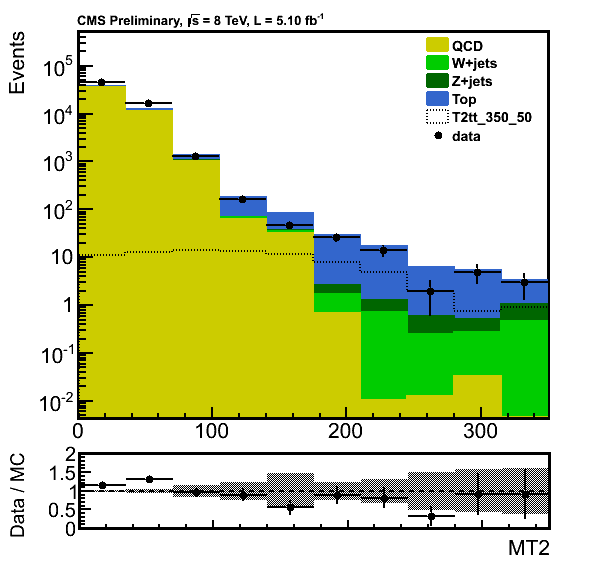
\includegraphics[width=0.49\textwidth]{figs/MT2.png}
\caption{\mttwo distribution after applying the full selection cuts.}
\label{fig:MT2}
\end{figure}
is used as a variable to search for SUSY.
To increase the power of the analysis, a multibinning approach is used.
We select 4 bins in \mttwo with the following edges 125, 150, 200, 250 and infinity.
Every \mttwo bin is devided to two bins with number of the reconstructed top quarks equal to 0 or greater than 0.
There will be 8 bins in the analysis. In this round of analysis, we try to emphasize the complementary role of this anaysis
for the common cut and count hadronic search for the direct stop production. Since this analysis, does not use the MET explicitly, 
it is more sensetive to the small mass differences between stop and LSP.
\section{Backgrounds}
\label{sect:bkg}
In this section, data driven methods are proposed and applied to estimate the contribution of the main background processes. 
Most of the methods are similar to what were used in the \mttwo analysis \cite{MT2_2011} with some minor changes which are explained
here.

